\documentclass[border=0.125cm]{standalone}
\usepackage{tikz}
\usetikzlibrary{positioning}
\usepackage{ifthen}
\usetikzlibrary{matrix,arrows.meta,quotes,shadows,decorations.pathreplacing,positioning,fadings}
\usepackage{cfr-lm}
\usetikzlibrary{arrows}
\input{arrowsnew}
\usetikzlibrary{arrows.meta}

\colorlet{mewnol}{blue!75!cyan}%
\colorlet{allanol}{blue!50!black}%

\begin{document}
		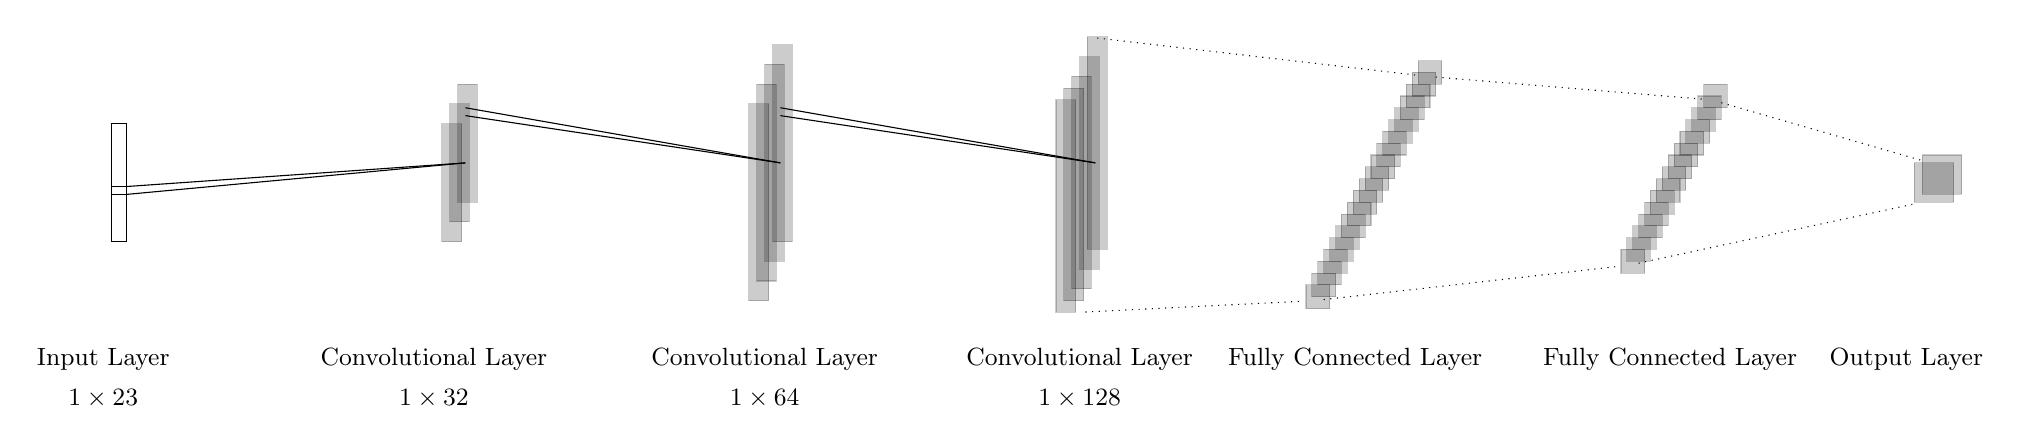
\begin{tikzpicture}
	% INPUT LAYER
	
	\node () at (1, -2) {\small Input Layer};	
	\node () at (1, -2.5) {\small $1\times23$};
	
	\draw (1.1,-0.5) rectangle (1.3,1.0);
	
	\draw (1.1,0.1) rectangle (1.3,0.2);
	
	\draw (1.3,0.1) -- (5.6,0.5);
	\draw (1.3,0.2) -- (5.6,0.5);
	
	% FIRST CONV LAYER
	\node () at (5.2,-2) {\small Convolutional Layer};
	\node () at (5.2, -2.5) {\small $1\times32$};
	
	%\draw[fill=black,opacity=0.2,draw=black] (3.25,0.75) -- (4.75,0.75) -- (4.75,2.25) -- (3.25,2.25) -- (3.25,0.75);
	\draw[fill=black,opacity=0.2,draw=black] (5.5,0.0) rectangle (5.75,1.5);
	\draw[fill=black,opacity=0.2,draw=black] (5.40,-0.25) rectangle (5.65,1.25);
	\draw[fill=black,opacity=0.2,draw=black] (5.3,-0.5) rectangle (5.55,1);
	
	\draw (5.6, 1.1) -- (9.6, 0.5);
	\draw (5.6, 1.2) -- (9.6, 0.5);
	
	% SECOND CONV LAYER
	\node () at (9.4,-2) {\small Convolutional Layer};
	\node () at (9.4, -2.5) {\small $1\times64$};
	
	\draw[fill=black,opacity=0.2,draw=black] (9.5,-0.5) rectangle (9.75,2);
	\draw[fill=black,opacity=0.2,draw=black] (9.40,-0.75) rectangle (9.65,1.75);
	\draw[fill=black,opacity=0.2,draw=black] (9.3,-1) rectangle (9.55,1.5);
	\draw[fill=black,opacity=0.2,draw=black] (9.2,-1.25) rectangle (9.45,1.25);
	
	\draw (9.6, 1.1) -- (13.6, 0.5);
	\draw (9.6, 1.2) -- (13.6, 0.5);
	
	% THIRD CONV LAYER
	\node () at (13.4,-2) {\small Convolutional Layer};
	\node () at (13.4, -2.5) {\small $1\times128$};
	
	\draw[fill=black,opacity=0.2,draw=black] (13.5,-0.6) rectangle (13.75,2.1);
	\draw[fill=black,opacity=0.2,draw=black] (13.40,-0.85) rectangle (13.65,1.85);
	\draw[fill=black,opacity=0.2,draw=black] (13.3,-1.1) rectangle (13.55,1.6);
	\draw[fill=black,opacity=0.2,draw=black] (13.2,-1.25) rectangle (13.45,1.45);
	\draw[fill=black,opacity=0.2,draw=black] (13.1,-1.4) rectangle (13.35,1.3);
	
	
	\node (lastConv-low) at (13.35, -1.4) {};
	\node (lastConv-high) at (13.5, 2.1) {};
	
	% FIRST FULLY CONNECTED LAYER
	\node () at (16.9,-2) {\small Fully Connected Layer};
	
	\foreach \m in {1,...,20}
			\draw[fill=black,opacity=0.2,draw=black] (16.5 + \m*0.075, -1.2 + \m*0.15) rectangle (16.2 + \m*0.075, -1.5 + + \m*0.15);
	
	\node (full1-low) at (16.3+0.075, -1.4 + 0.15) {};
	\node (full1-high) at (16.3+0.075*20, -1.4 + 0.15*20) {};
	
	% SECOND FULLY CONNECTED LAYER
	\node () at (20.9,-2) {\small Fully Connected Layer};
	
	\foreach \m in {1,...,15}
		\draw[fill=black,opacity=0.2,draw=black] (20.5 + \m*0.075, -0.75 + \m*0.15) rectangle (20.2 + \m*0.075, -1.05 + + \m*0.15);
		
	\node (full2-low) at (20.3+0.075, -0.95 + 0.15) {};
	\node (full2-high) at (20.3+0.075*15, -0.95 + 0.15*15) {};
	
	% OUTPUT LAYER
		\node () at (23.9,-2) {\small Output Layer};
		\draw[fill=black,opacity=0.2,draw=black]  (24, 0) rectangle (24.5, 0.5);
		\draw[fill=black,opacity=0.2,draw=black]  (24.1, 0.1) rectangle (24.6, 0.6);
		\node (out-low) at (24.1, 0) {};
		\node (out-high) at (24.2,0.5) {};
		
	\draw[dotted] (full1-low) -- (full2-low);
	\draw[dotted] (full1-high) -- (full2-high);
	\draw[dotted] (lastConv-low) -- (full1-low);
	\draw[dotted] (lastConv-high) -- (full1-high);
	\draw[dotted] (full2-low) -- (out-low);
	\draw[dotted] (full2-high) -- (out-high);
	\end{tikzpicture}
\end{document}